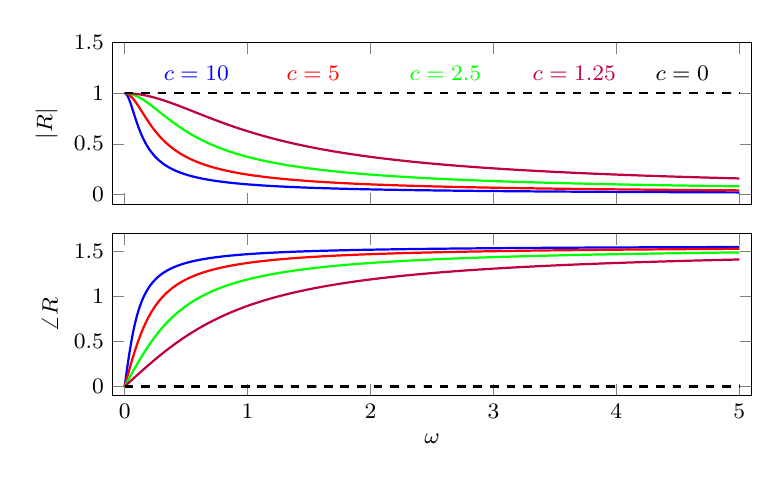
\begin{tikzpicture}[scale=1]
	\footnotesize
	\begin{axis}[
		at={(0,0.2\textwidth)},
		width=0.8\textwidth,
		height=0.3\textwidth,
		ylabel = {$|R|$},
		xticklabel=\empty,
		xmax=5.1,
		xmin=-0.1,
		ymax=1.5,
		ymin=-0.1,  
		samples=500]
		
		
		\def\k{1};
		\def\cA{10};
		\def\cB{5};
		\def\cC{2.5};
		\def\cD{1.25};		
		\def\cE{0};		
		
		\addplot[blue, thick, domain=0:5] (x, {1/sqrt(\k^2 + (x*\cA)^2)});
		\addplot[red, thick, domain=0:5] (x, {1/sqrt(\k^2 + (x*\cB)^2)});
		\addplot[green, thick, domain=0:5] (x, {1/sqrt(\k^2 + (x*\cC)^2)});
		\addplot[purple, thick, domain=0:5] (x, {1/sqrt(\k^2 + (x*\cD)^2)});
		\addplot[black, dashed, thick, domain=0:5] (x, {1/sqrt(\k^2 + (x*\cE)^2)});
	
		
		\node at (axis cs: 0.25, 1.2) [blue,anchor=west] {$c=10$};
		\node at (axis cs: 1.25, 1.2) [red,anchor=west] {$c=5$};
		\node at (axis cs: 2.25, 1.2) [green,anchor=west] {$c=2.5$};
		\node at (axis cs: 3.25, 1.2) [purple,anchor=west] {$c=1.25$};
		\node at (axis cs: 4.25, 1.2) [black,anchor=west] {$c=0$};
		
	\end{axis}

	\begin{axis}[
	at={(0,0.\textwidth)},
	width=0.8\textwidth,
	height=0.3\textwidth,
	xlabel={$\omega$},
	ylabel = {$\angle R$},
	xmax=5.1,
	xmin=-0.1,
	ymax=1.7,
	ymin=-0.1,  
	samples=500]
	
	
	\def\k{1};
	\def\cA{10};
	\def\cB{5};
	\def\cC{2.5};
	\def\cD{1.25};		
	\def\cE{0};		
	
	\addplot[blue, thick, domain=0:5] (x, {rad(atan(x*\cA/\k))});
	\addplot[red, thick, domain=0:5] (x, {rad(atan(x*\cB/\k))});
	\addplot[green, thick, domain=0:5] (x, {rad(atan(x*\cC/\k))});
	\addplot[purple, thick, domain=0:5] (x, {rad(atan(x*\cD/\k))});
	\addplot[black, dashed, thick, domain=0:5] (x, {rad(atan(x*\cE/\k))});
	
	
\end{axis}
	
\end{tikzpicture}